\section{Maximum Power Point Tracking techniques\label{MPPTalgo}}

There is a variety of different techniques for finding the maximum power point. Therefore, two different MPPT algorithms will be described in this project, otherwise it would go beyond the scope of this work. These two methods are the Perturb and Observe (P\&O) and constant voltage. P\&O is one of the most used algorithm in commercial PV panels \cite{Dezso}. On the other hand, constant voltage has been selected as an example for other less used methods. Each MPPT algorithm will be described based on a flow chart. 

\subsection{Constant voltage}
Empirical experiments have shown that the voltage of the MPP has a linear dependence on the open-circuit voltage at different ambient conditions\cite{flowchartVC}.

\begin{equation} \label{voltage_MPP}
V_{MPP} = k \cdot V_{OC}	
\end{equation} 

In equation \ref{voltage_MPP}, $k$ represents a constant that depends on the characteristics of the respective PV panel. To determine the value of $k$, the MPP voltage ($V_{MPP}$) and the open-circuit voltage ($V_{OC}$) must be empirical recorded for each temperature and solar irradiation before final implementation. According to different papers, this value lies between 70\% and 80\% of $V_{OC}$.\cite{MPPTResearch}\cite{MPPTConstV}

\todo{I change the text. Now the text is like in reference 18. So we do not need the flow chart here.}

%The $k$ look-up table calculation algorithm starts with the recording of $V_{OC}$ and a predetermined $k$-value. In each iteration step $V_{MPP}$ is calculated first. After this, the operating voltage is compared with the calculated $V_{MPP}$. If the voltage is not equal, the constant $k$ is changed for the next iteration step to track the MPP. When the algorithm has reached the MPP, the algorithm is stopped, as it is showed in the flow chart in the figure \ref{fcconstantvoltage}. \cite{flowchartVC}

The advantage of using constant voltage is that only the voltage is measured and the system is controlled by a simple control loop. Therefore, implementation costs are low compared to P\&O. The use of PV modules with the constant voltage as MPPT algorithm is only possible in regions with low temperature fluctuations. The reason for this disadvantage is that the point of the MPP varies greatly with strong temperature fluctuations and the assumption of linear dependence is no longer valid. In addition, it is not possible to find the MPP with the algorithm if the PV module is partially shaded. Another disadvantage is the effort of calculating the optimal $k$ for different levels of irradiance and temperature is very high.\cite{flowchartVC} \cite{MPPTConstV}


\begin{figure}[H]
	\begin{center}
		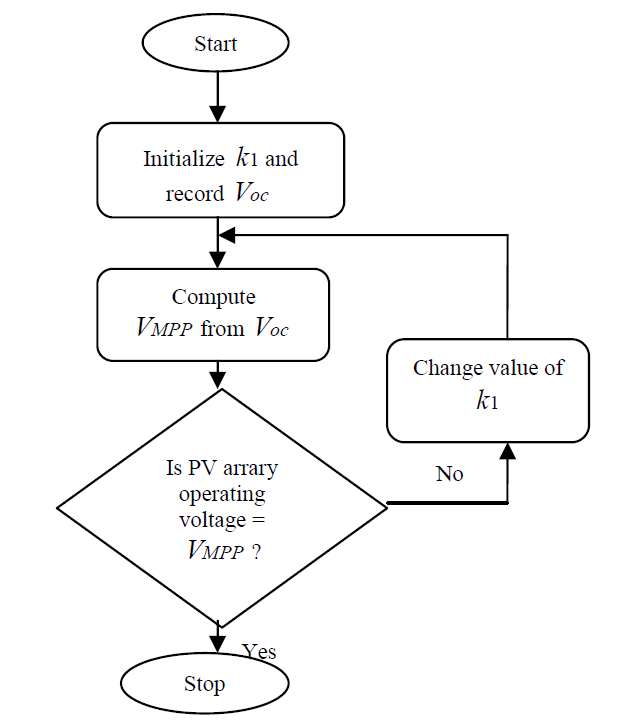
\includegraphics[width=0.5\textwidth]{../Pictures/P1/Flow_chart/Flow_chart_constant_voltage}
		\caption{Flow chart for the constant voltage $k$-parameter look-up table calculation \cite{flowchartVC}. }
		\label{fcconstantvoltage}
	\end{center}	
\end{figure}


\subsection{Perturb and observe}
With the P\&O method, the currently measured power is periodically compared with the previous power. If the measured power is greater than the power from the previous measurement, the algorithm is moving in the right direction to the MPP. If a power reduction is detected after the comparison, the algorithm is moving away from the MPP. The next step is the identification of a voltage increase or reduction to regulate the voltage for getting the MPP voltage.
This depends on which side of the MPP the algorithm is working.
On the left side of the MPP the increment of power with respect to voltage is greater than 0 while on the right side it is less than 0, this behavior is described by the following equations. \cite{AN1521_MC}

\begin{equation} \label{PO1}
\frac{\Delta P}{\Delta V} = 0 ,\; at\; MPP 
\end{equation} 
\begin{equation} \label{PO2}
\frac{\Delta P}{\Delta V} > 0 ,\; left\; side\; from\; MPP 
\end{equation}
\begin{equation} \label{PO3}
\frac{\Delta P}{\Delta V} < 0 ,\; right\; side\; from\; MPP
\end{equation}


The flow chart in figure \ref{fcperturbandobserve} illustrates this method. The classical algorithm uses a fixed step to change the voltage. When the MPP is reached, the algorithm oscillates around this point. The output of the algorithm can be both duty cycle or voltage reference, in the figure voltage reference is used. \cite{flowchartVC}

One of the advantages of the P\&O algorithm is that the required computing power is  low, in its simplest implementation. The algorithm contains the calculation of the power and the comparison with the previous power for each step. There is a disadvantage when the algorithm is near to the MPP since, at this point, the algorithm oscillates around it, so that the MPP cannot be reached accurately. The oscillation depends on the value of the perturb step. If the fixed step value is high, the MPP will be tracked quickly. However, the oscillation around the MPP is higher, which reduces the efficiency of the PV panel. The advantage of a small step value is that the oscillations are reduced, but it takes more time to reach the MPP. \cite{AN1521_MC}

\begin{figure}[H]
	\begin{center}
		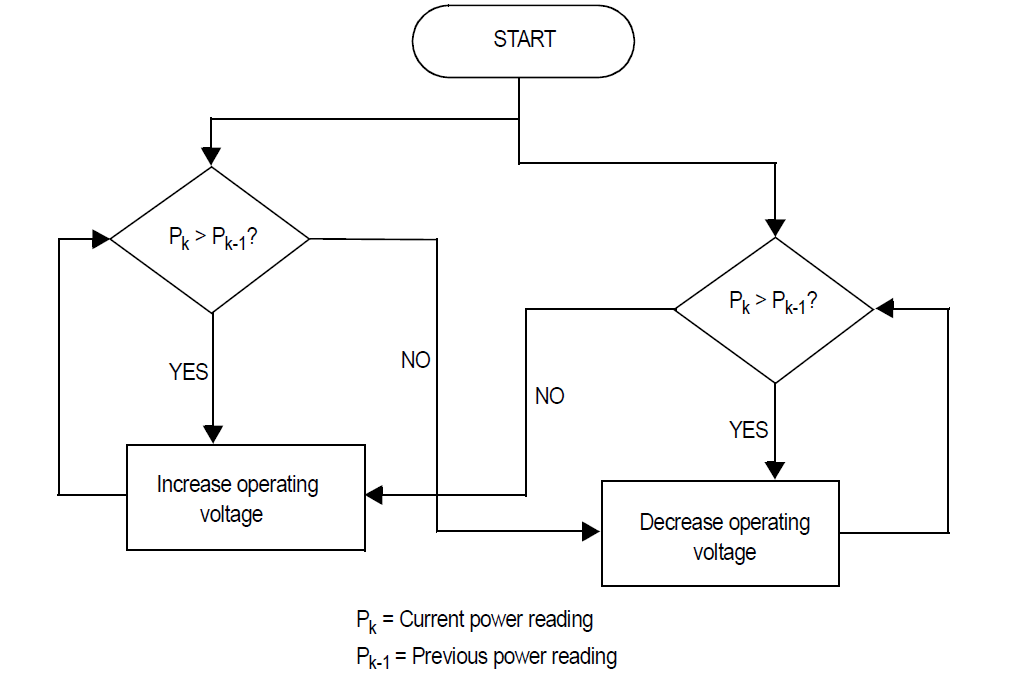
\includegraphics[width=0.8\textwidth]{../Pictures/P1/Flow_chart/flow_chart_perturb_observe}
		\caption{Flow chart for the conventional P\&O algorithm \cite{PerturbObserveFC}.}
		\label{fcperturbandobserve}
	\end{center}	
\end{figure}

\iffalse
\subsection{Incremental conductance}
The approach of incremental conductance is that the MPP is at the position where the derivative of the power with respect to the voltage is 0, see figure \ref{fig:mpp}. On the left side of the MPP the increment of power with respect to voltage is greater than 0 while on the right side it is less than 0, this behavior is described by the following equations. \cite{AN1521_MC}

\begin{equation} \label{Inccond1}
\frac{dP}{dV} = 0 ,\; at\; MPP 
\end{equation} 
\begin{equation} \label{Inccond2}
\frac{dP}{dV} > 0 ,\; left\; side\; from\; MPP 
\end{equation}
\begin{equation} \label{Inccond3}
\frac{dP}{dV} < 0 ,\; right\; side\; from\; MPP
\end{equation}

The algorithm compares the incremental conductance with the previous one to increase (left side of MPP) or decrease (right side of MPP) the voltage. After the MPP has been reached, the algorithm is stopped. Thus, there will be no oscillation around the MPP. If a change in the current is detected, the algorithm starts to find the MPP again, as you can see in the flow chart in figure \ref{fcinccon}. \cite{AN1521_MC}

An advantage of this MPPT algorithm is that it can reach exactly the MPP. This increases the efficiency of the PV panel. As with the P\&O algorithm, a fixed value is used to change the voltage. If the value is high, the probability is higher that the algorithm oscillates around the MPP. 
Two sensors, for the voltage and the current, are used for the implementation of this method. In addition, the microcontroller requires a higher computing power than with the P\&O algorithm. This is because more commands are called up during an iteration step. The costs for the algorithm development and microcontroller are higher compared to the other two algorithms. \cite{AN1521_MC}

\begin{figure}[H]
	\begin{center}
		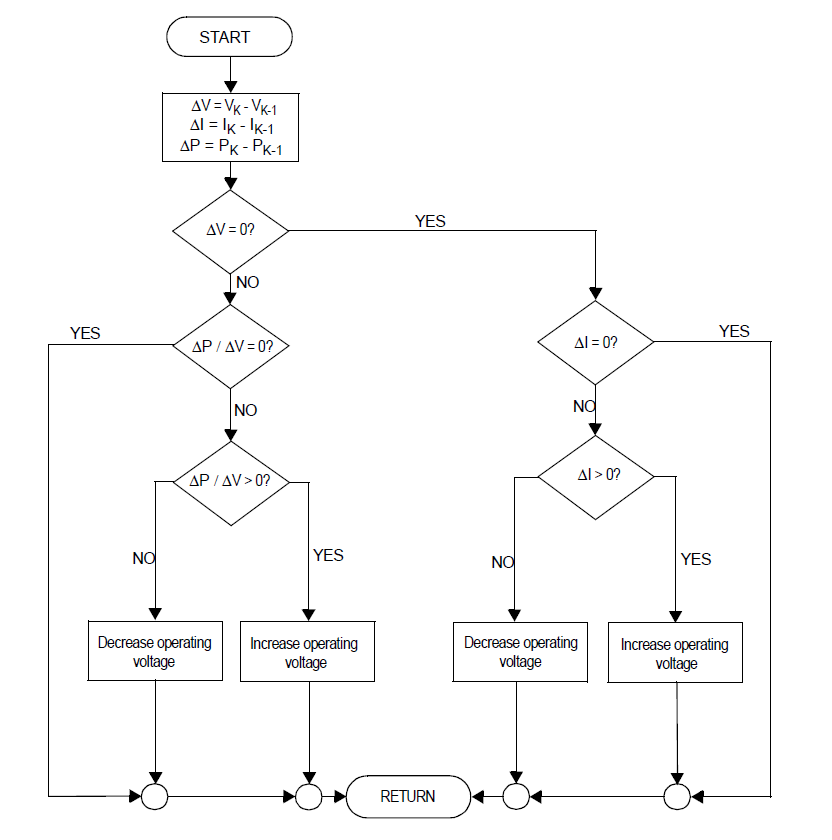
\includegraphics[width=0.8\textwidth]{../Pictures/P1/Flow_chart/flow_chart_incremental_conductance}
		\caption{Flow chart for the incremental conductance algorithm \cite{AN1521_MC}.}
		\label{fcinccon}
	\end{center}	
\end{figure}


%  not delete this tabel because we can use it in the presentation
%Table \ref{summaryMPPT} gives an overview of the advantages and disadvantages of the different algorithms.
%%\begin{table}[H] 	
%	\centering 
%	\begin{tabular}  {|>{\centering}m{2cm}|>{\centering}m{2cm}|>{\centering}m{2cm}|>{\centering}m{2cm}|>{\centering}m{2cm}|>{\centering}m{2cm}|}
%		\hline
%		\rowcolor{lightgray}						 \textbf{MPPT Algorithm} & 	
%		\textbf{Sensed Parameters} &
%		\textbf{Micro-controller Computation} &
%		\textbf{Complexity}&
%		\textbf{Reliability}	&
%		\textbf{Overall Cost}
%		\tabularnewline  \hline
%		Constant voltage 	& Voltage 		& Absent/Low &  Very simple & Not accurate & Low 										\tabularnewline \hline
%		Perturb and observe & Voltage + Current  & Low  &  Medium & Not so much accurate & Low/ Medium 		\tabularnewline \hline
%		Incremental conductance & Voltage + Current & Medium &  Medium/ High & Accurate and operate at MPP & Low/ Medium	\tabularnewline	\hline
%	\end{tabular} \label{tab:summaryMPPT}
%	\caption{Summary  of the MPPT algorithm \cite{flowchartVC} }
%
%\end{table}
\fi


